%!TEX root = start.TEX

%----------------Resultados de la tesis----------


\section{Resultados de la tesis}

\frame{
\begin{block}
{\Large{Resultados de la tesis}}
\end{block}
%\vskip 0.5cm
\begin{itemize}
	\item<1->Indicadores:
	\begin{itemize}
	\item Efectividad(Prop. Verdaderos Pos): {$PVP= \frac{Verdaderos\,Positivos}{{Verdaderos\,Positivos} + {Falsos\,Negativos}}$}
	\vskip 0.2cm
	\item Especificidad(Prop. Verdaderos Neg): {$PVN= \frac{Verdaderos\,Negativos}{{Verdaderos\,Negativos} + {Falsos\,Positivos}}$}
	\vskip 0.2cm
	\item Valor Predictivo Positivo (Precisión): {$PPV = \frac{Verdaderos\,Positivos}{{Verdaderos\,Positivos}+{Falsos\,Positivos}}$}
	\vskip 0.2cm
	\item Acuracia (Exactitud): {$ACC= \frac{Verdaderos\,Positivos+Verdaderos\,Negativos}{Total\,de\,Imagenes}$}
	\end{itemize}
	\vskip 0.2cm	
	\item<2->Donde:
	\begin{itemize}
		\item[--] Verdaderos Positivos: Imágenes correctamente indentificadas.
		\item[--] Falsos Positivos: Imágenes incorrectamente identificadas.
		\item[--] Verdaderos Negativo:Imágenes correctamente rechazadas.
		\item[--] Falsos Negativos:Imágenes incorrectamente rechazadas.
	\end{itemize}
	
\end{itemize}
}

\frame{
\begin{block}
{\Large{Resultados de la tesis}}
\end{block}
%\vskip 0.5cm
\begin{itemize}
	\item<1->Utilizando los anteriores indicadores, podemos obtener dos más:
	\begin{itemize}
		\item Curvas ROC : Relación entre Efectividad y Especificidad
		\vskip 0.2cm	
		\item Curvas PR  : Relación entre Precisión y Efectividad(Recall)
		\vskip 0.2cm	
	\end{itemize}
	\vskip 0.3cm
	\item<2->Las curvas ROC se utilizan normalmente para estudiar la salida de un clasificador. Para dibujarlas se construye la línea convexa formada por los puntos (PFP, PVP) de los clasificadores que se estén evaluando. La curva más cercana a los bordes izquierdo y superior en el espacio ROC, es la prueba más acertada porque significa que hay mayor acierto. 
	\vskip 0.3cm
	\item<3->El mejor sistema de entrenamiento es el que produce un conjunto de clasificadores que maximice el área bajo la curva(AUC - Area Under the Curve)\citep{SandovalCereza}.

	%La curva que más se acerque a la diagonal de 45 grados en el espacio ROC, es la prueba menos acertada.
\end{itemize}
}
%------------------------------------------------------------------------------------------------------------------------------------------

\frame{
\begin{block}
{\Large{Resultados de la tesis - Señales de Tránsito de Alemania}}
\end{block}
%\vskip 0.5cm

	\begin{table}[H]
			\begin{center}
			\caption{\small{Indicadores de los 5 modelos entrenados en el Dataset - Alemania}}
			\vspace{1.1em}
			\begin{tabular}{c|c|c|c|c|c|}
			\cline{2-6}
			                                 & \textbf{Modelo A} & \textbf{Modelo B} & \textbf{Modelo C} &\textbf{ Modelo D} & \textbf{Modelo E} \\ \hline
			\multicolumn{1}{|c|}{\textbf{PVP}}        & 96.14     & 98.35       & 98.08       & 98.37       & 98.61       \\ \hline
			\multicolumn{1}{|c|}{\textbf{PVN}}        & 99.93     & 99.96       & 99.96       & 99.96       & 99.97       \\ \hline
			\multicolumn{1}{|c|}{\textbf{PPV}}        & 95.69     & 97.52       & 97.57       & 97.78       & 98.01      \\ \hline
			\multicolumn{1}{|c|}{\textbf{AUC-PR}}     & 94.31     & 96.88       & 96.60       & 96.93       & 97.30       \\ \hline
			\multicolumn{1}{|c|}{\textbf{AUC-ROC}}    & 98.04     & 99.15       & 99.02       & 99.17       & 99.29       \\ \hline
			\multicolumn{1}{|c|}{\textbf{ACC}}        & 97.08     & 98.41       & 98.27       & 98.43       & 98.62       \\ \hline
			\end{tabular}
			\end{center}
		\end{table}
}



\frame{
\begin{block}
{\Large{Señales de Tránsito de Alemania}}

\end{block}
%\vskip 0.5cm

	\begin{figure}[H]
		\begin{center}
		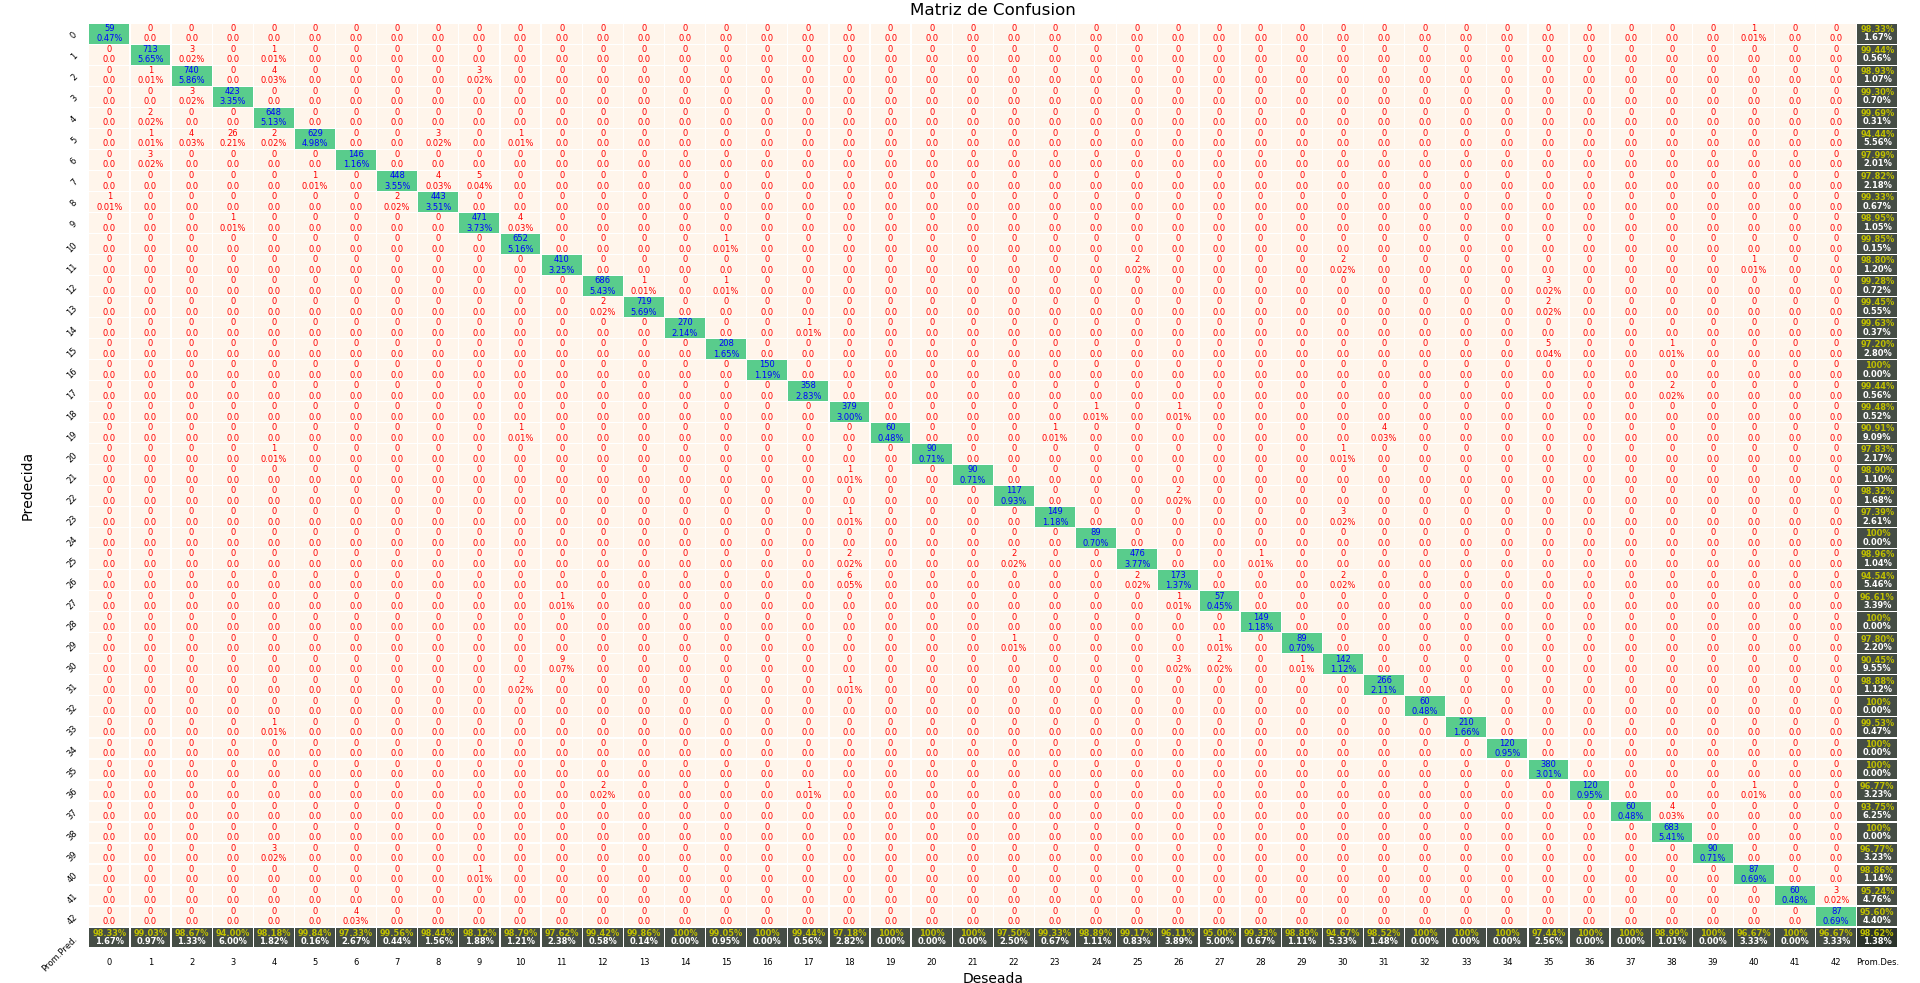
\includegraphics[width=\textwidth, height=1.2\textheight,keepaspectratio]{images/desarrollo/testResults/german/model_A_A_1} 
		\end{center}
		\begin{center}
		\caption{\tiny{Matriz de Confusión del Modelo E - Dataset de imágenes de Alemania}}
		\vspace{-1em}
		{\tiny {Fuente: Elaboración propia}}
		\end{center}
		%\vspace{-1.5em}
	\end{figure}
}


\frame{
\begin{block}
{\Large{Señales de Tránsito de Alemania}}

\end{block}
%\vskip 0.5cm
	\begin{figure}[H]
		\begin{center}
		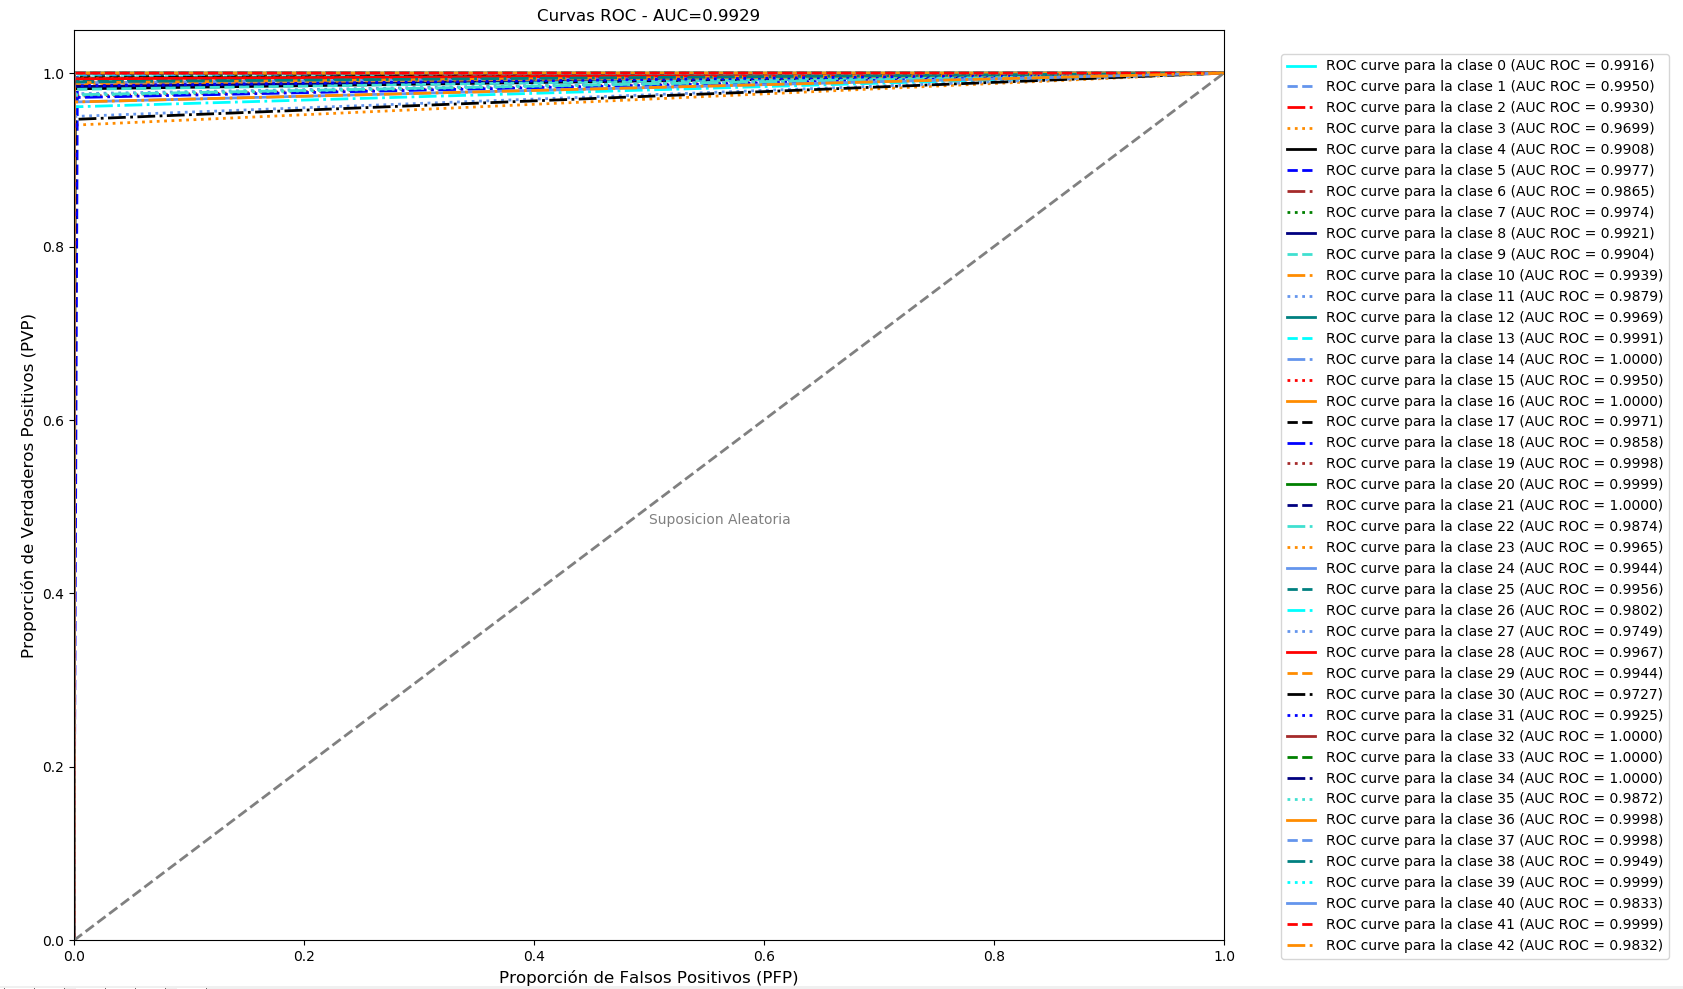
\includegraphics[width=\textwidth, height=0.7\textheight,keepaspectratio]{images/desarrollo/testResults/german/ROC_curve_modelE} 
		\end{center}
		\vspace{-1em}
		\begin{center}
		\caption{\tiny{Área debajo de la Curva ROC del Modelo E - Dataset de imágenes de Alemania}}
		\vspace{-1em}
		{\tiny {Fuente: Elaboración propia}}
		\end{center}
	\end{figure}
}

\frame{
\begin{block}
{\Large{Señales de Tránsito de Alemania}}

\end{block}
%\vskip 0.5cm
	\begin{figure}[H]
		%\begin{center}
		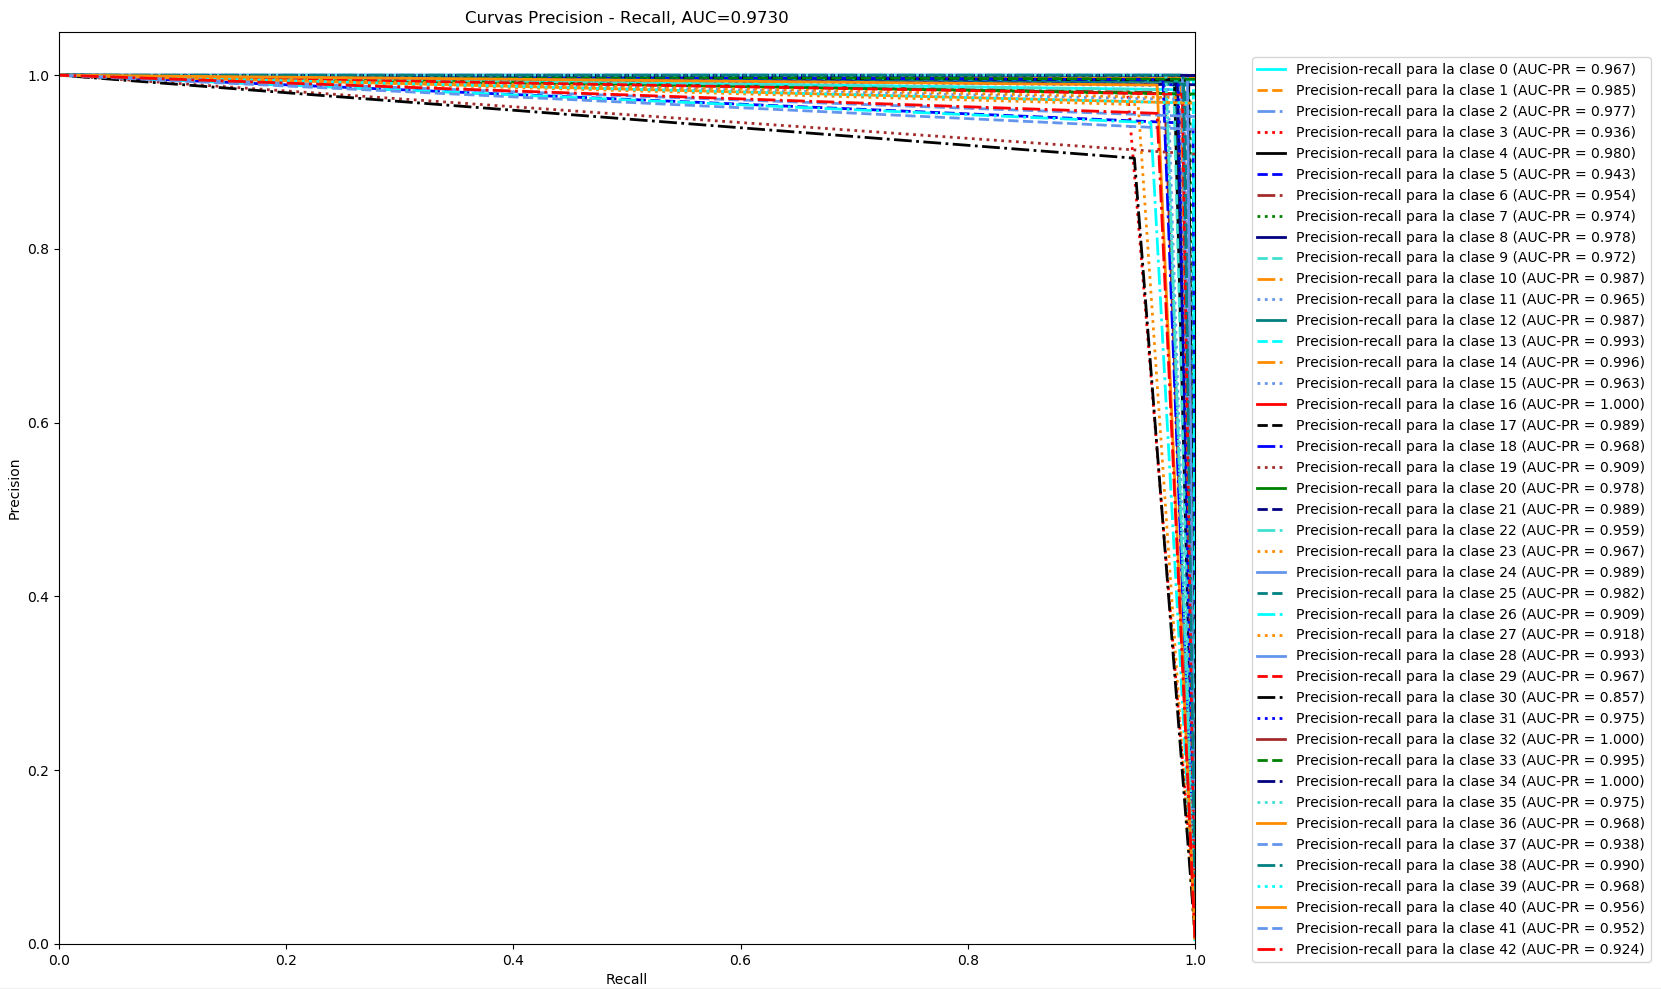
\includegraphics[width=\textwidth, height=0.7\textheight,keepaspectratio]{images/desarrollo/testResults/german/PR_curve_modelE} 
		%\end{center}
		\vspace{-1em}
		\begin{center}
		\caption{\tiny{Área debajo de la Curva PR del Modelo E - Dataset de imágenes de Alemania}}
		\vspace{-1em}
		{\tiny{Fuente: Elaboración propia}}
		\end{center}
		
	\end{figure}	
}



%------------------------------------------------------------------------------------------------------------------------------------------


\frame{
\begin{block}
{\Large{Resultados de la tesis - Señales de Tránsito de Perú}}
\end{block}
%\vskip 0.5cm

	\begin{table}[H]
			\begin{center}
			\caption{\small{Indicadores de los 5 modelos entrenados en el Dataset - Perú}}
			\vspace{1.1em}
			\begin{tabular}{c|c|c|c|c|c|}
			\cline{2-6}
			                                 & \textbf{Modelo A} & \textbf{Modelo B} & \textbf{Modelo C} &\textbf{ Modelo D} & \textbf{Modelo E} \\ \hline
			\multicolumn{1}{|c|}{\textbf{PVP}}        & 95.78     & 99.16       & 99.26       & 98.97       & 99.83       \\ \hline
			\multicolumn{1}{|c|}{\textbf{PVN}}        & 99.44     & 99.91       & 99.92       & 99.86       & 99.97       \\ \hline
			\multicolumn{1}{|c|}{\textbf{PPV}}        & 96.75     & 99.40       & 99.49       & 99.31       & 99.86       \\ \hline
			\multicolumn{1}{|c|}{\textbf{AUC-PR}}     & 94.06     & 98.98       & 99.09       & 98.54       & 99.68       \\ \hline
			\multicolumn{1}{|c|}{\textbf{AUC-ROC}}    & 97.62     & 99.51       & 99.60       & 99.42       & 99.90       \\ \hline
			\multicolumn{1}{|c|}{\textbf{ACC}}        & 96.74     & 99.45       & 99.51       & 98.21       & 99.83       \\ \hline
			\end{tabular}
			\end{center}
		\end{table}
}



\frame{
\begin{block}
{\Large{Señales de Tránsito de Perú}}

\end{block}
%\vskip 0.5cm

	\begin{figure}[H]
		\begin{center}
		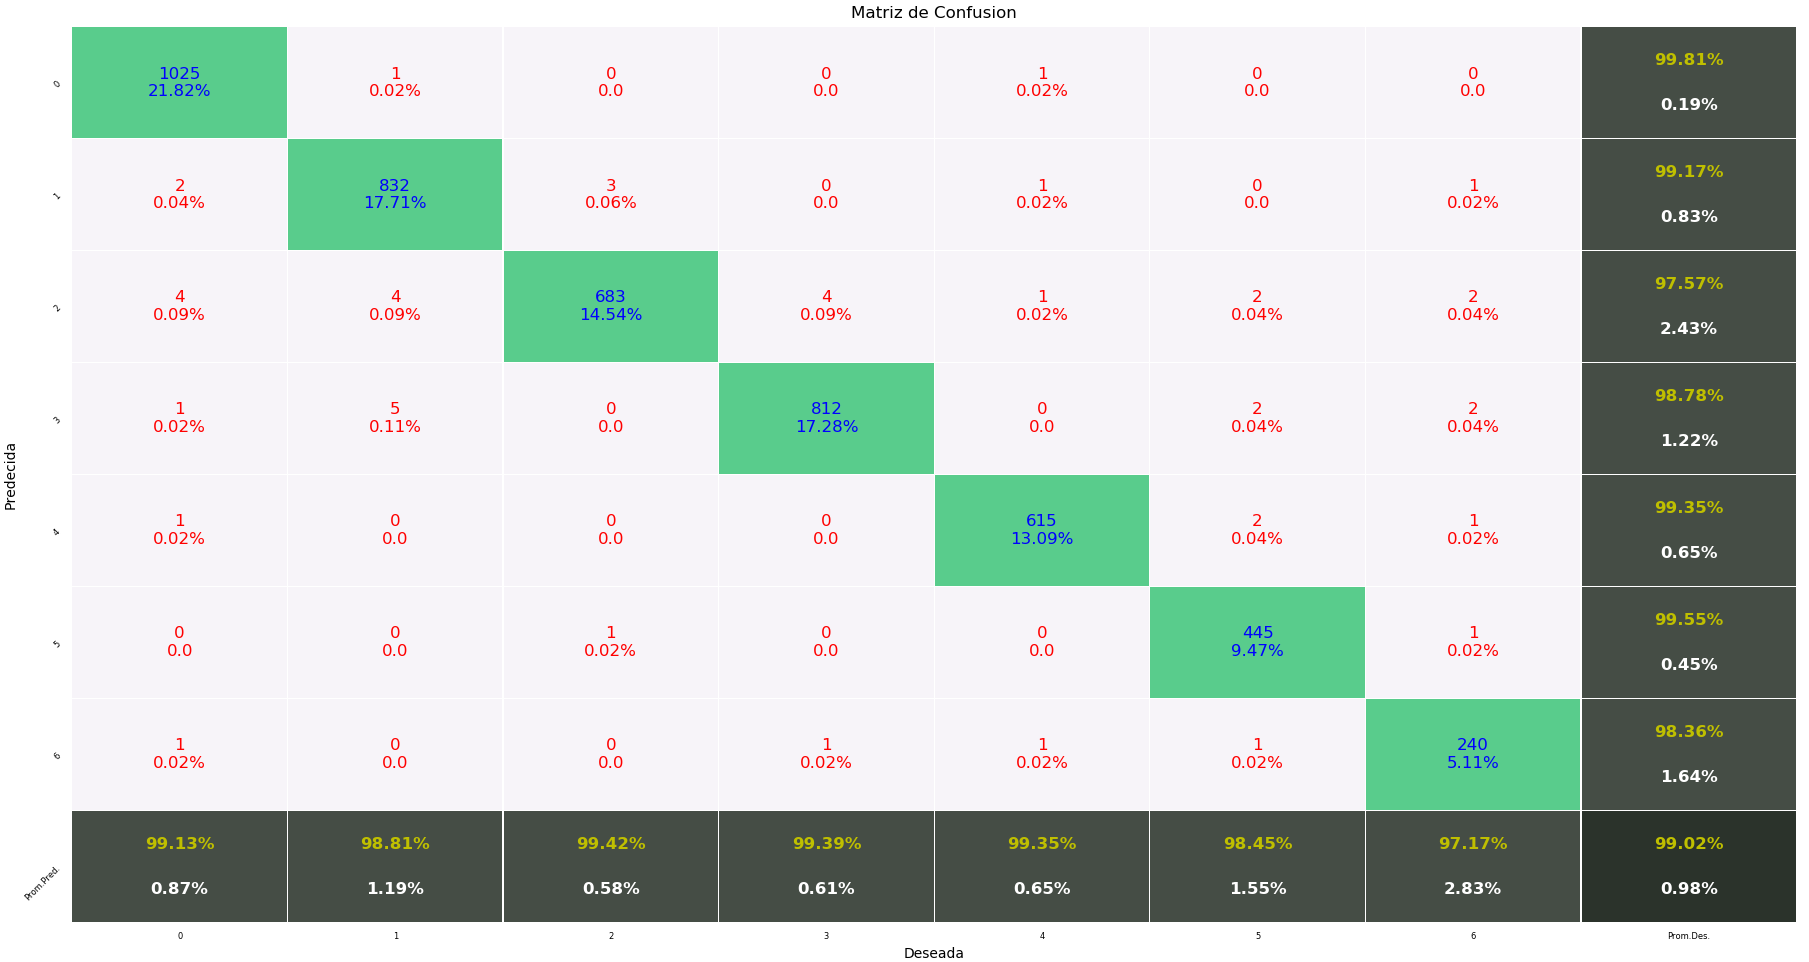
\includegraphics[width=\textwidth, height=0.7\textheight,keepaspectratio]{images/desarrollo/testResults/peru/modelE} 
		\end{center}
		\vspace{-1em}
		\begin{center}
		\caption{\tiny{Matriz de Confusión del Modelo E - Dataset de imágenes de Perú}}
		\vspace{-1em}
		{\tiny {Fuente: Elaboración propia}}
		\end{center}
		%\vspace{-1.5em}
	\end{figure}
}


\frame{
\begin{block}
{\Large{Señales de Tránsito de Perú}}

\end{block}
%\vskip 0.5cm
	\begin{figure}[H]
		\begin{center}
		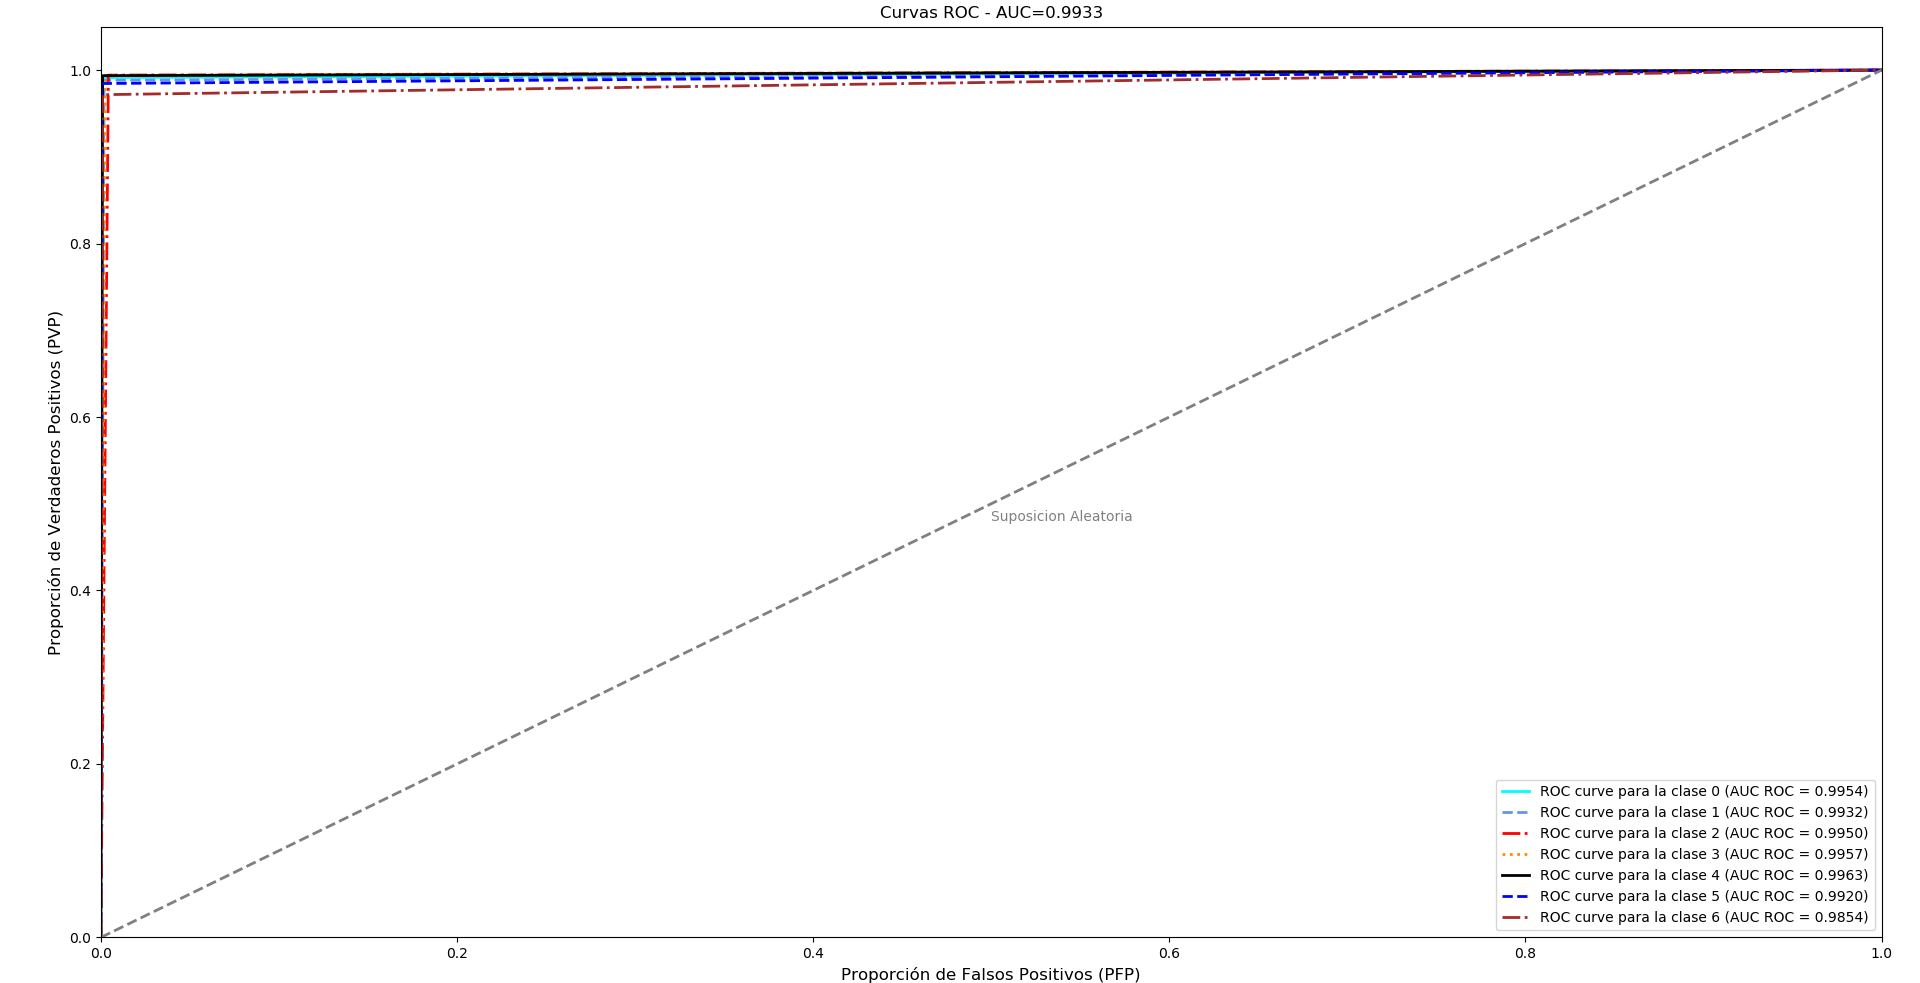
\includegraphics[width=\textwidth, height=0.7\textheight,keepaspectratio]{images/desarrollo/testResults/peru/ROC_curve_modelE} 
		\end{center}
		\vspace{-1em}
		\begin{center}
		\caption{\tiny{Área debajo de la Curva ROC del Modelo E - Dataset de imágenes de Perú}}
		\vspace{-1em}
		{\tiny {Fuente: Elaboración propia}}
		\end{center}
	\end{figure}
}

\frame{
\begin{block}
{\Large{Señales de Tránsito de Perú}}

\end{block}
%\vskip 0.5cm
	\begin{figure}[H]
		%\begin{center}
		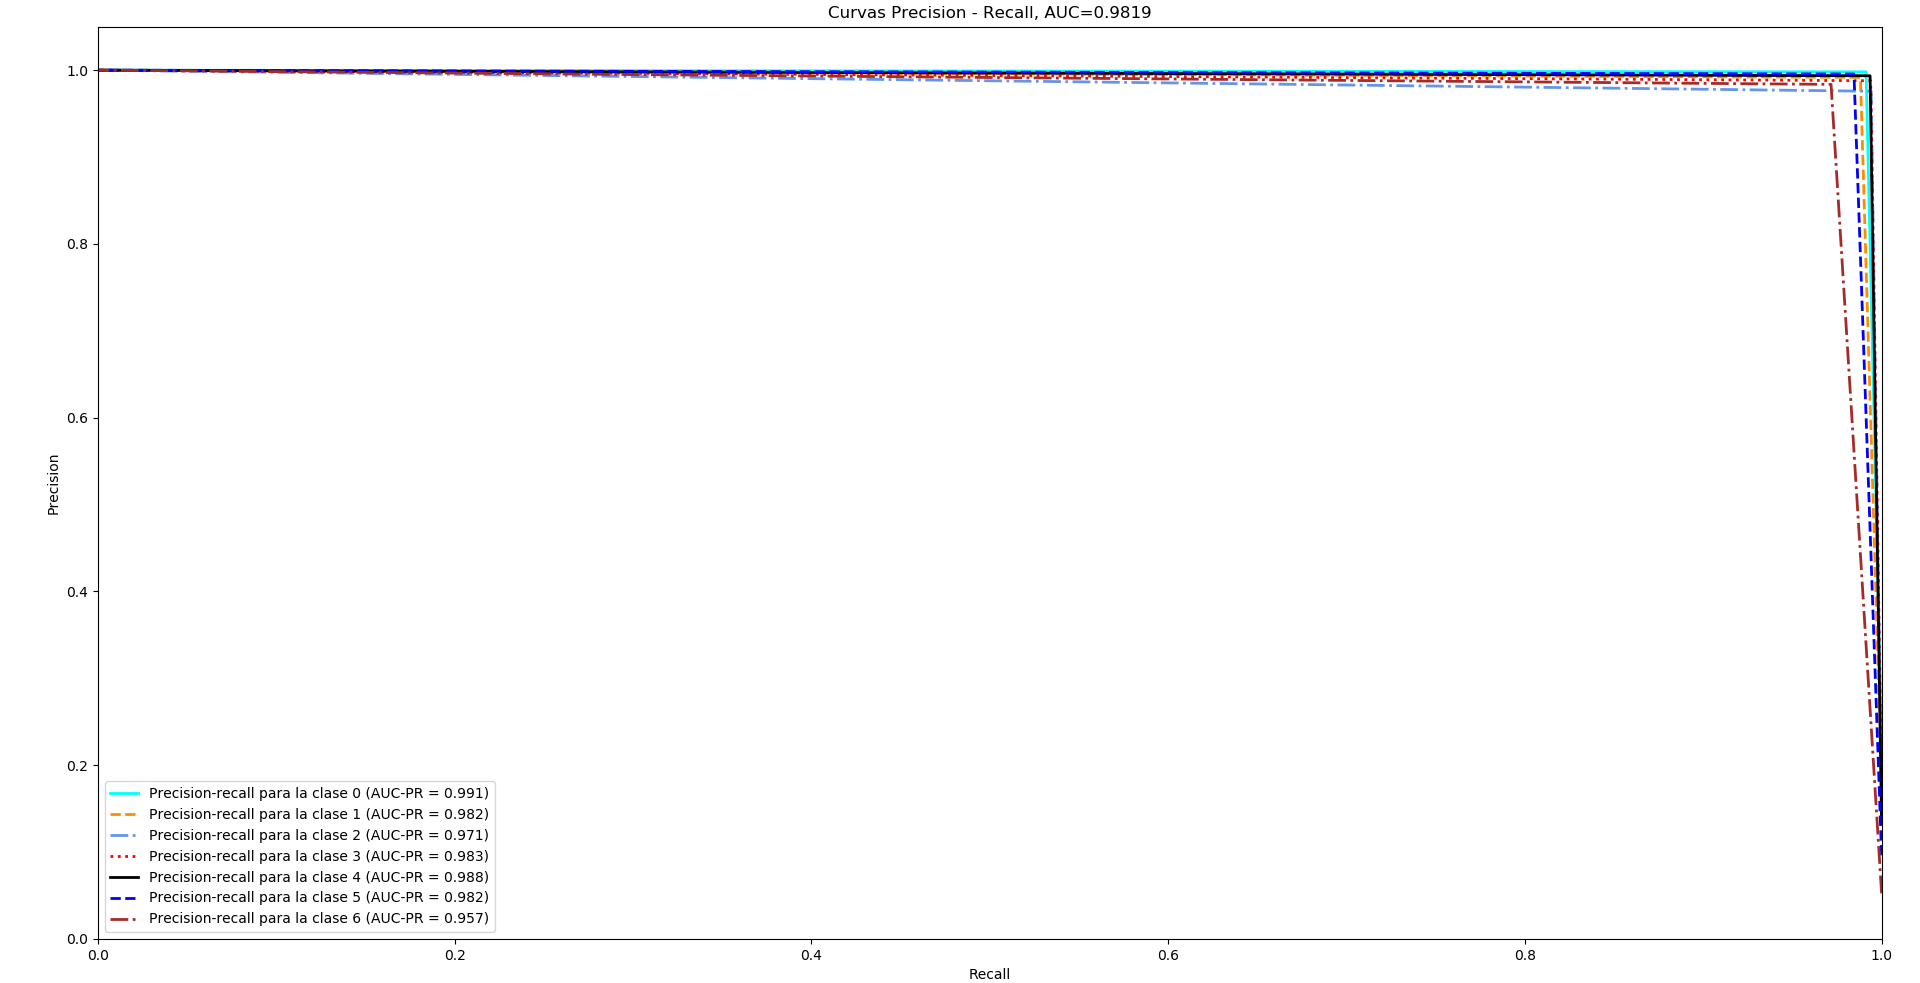
\includegraphics[width=\textwidth, height=0.7\textheight,keepaspectratio]{images/desarrollo/testResults/peru/PR_curve_modelE} 
		%\end{center}
		\vspace{-1em}
		\begin{center}
		\caption{\tiny{Área debajo de la Curva PR del Modelo E - Dataset de imágenes de Perú}}
		\vspace{-1em}
		{\tiny{Fuente: Elaboración propia}}
		\end{center}
		
	\end{figure}	
}



%------------------------------------------------------------------------------------------------------------------------------------------


\section{Consideraciones finales}


\frame{
\begin{block}
{\Large{Consideraciones finales}}
\end{block}
\vskip 0.5cm
	\begin{itemize}
		\item<1-> {\bf Conclusiones:}
		\begin{itemize}
		\item<2-> El objetivo general que trata sobre implementar un modelo basado en el aprendizaje profundo de redes neuronales convolucionales para reconocer automáticamente señales de tránsito vehicular fue conseguido a través del Modelo E.
		\vskip 0.3cm
		\item<3->El modelo final obtenido compuesto principalmente de 4 capas convolucionales, 2 capas totalmente conectadas, funciones de escala múltiple y cerca de 76393 neuronas(Sección 3.2.1.5 - Diseño E), contribuye en el reconocimiento de señales de Tránsito Alemanas con una tasa de acierto del {\bf 98.62\%}, mucho mejor que el resultado obtenido por \citep{Ayuque2016} - 95.29\% y mucho más próximo al estado del arte (99.46\% - \citep{Ciresan}).
		\vskip 0.3cm
		\item<4->La investigación ofrece para futuras investigaciones, un dataset de señales de Tránsito del Perú compuesto por 31314 imágenes distribuidas en 7 categorías(Sección 3.1.4.2). Para dicho dataset, el modelo con las mismas configuraciones también permite obtener un {\bf alto grado de acierto (99.83\%)} tras analizar 4698 imágenes. 
	\end{itemize}
\end{itemize}
}

\frame{
\begin{block}
{\Large{Consideraciones finales}}
\end{block}
\vskip 0.5cm
	\begin{itemize}
		\item<1-> {\bf  Trabajos futuros:}
		\begin{itemize}
		\item<2->El modelo puede ser ampliado a tener muchas más capas convolucionales y totalmente conectadas para poder experimentar si existe una mejora en los resultados. Además se recomienda obtener muchas más imágenes para exceder el rendimiento humano, \citep{Goodfellow-et-al-2016}
		\vskip 0.3cm
		\item<3->Ampliar el dataset de señales de tránsito del Perú con la finalidad de abarcar más categorías, ya que se tiene confianza por lo mostrado con el dataset de Alemania que el modelo es robusto para soportar mayor cantidad de estas.
		\vskip 0.3cm
		\item<4->Se sugiere integrar el modelo obtenido en un sistema más general que primero localize las señales de tránsito en escenas que abarcan más de una señal de tránsito, para luego proceder a su reconocimiento (multi-clasificación).
		\end{itemize}
\end{itemize}
}

